\begin{frame}{Side-channel attacks}
    \begin{itemize}
        \item Side-channel analysis attacks target cryptographic implementations passively.
       \item The attacks exploit the possibility of the attacker observing the physical characteristics of a device that is running the cryptographic algorithm.
        \item The attacker obtains the side-channel information, e.g. power consumption, execution time, then utilizes such information to recover the secret key.
     \item  In this course, we will mainly focus on power analysis attacks that exploit power consumption information.
      \item The attack methodologies can be used in a similar manner when electromagnetic emanation (EM) is analyzed.
    \end{itemize}
\end{frame}

\begin{frame}{Device under test (DUT)}
    \begin{itemize}
        \item The device that we take measurement of is called the \textit{device under test (DUT)}
        \begin{itemize}
            \item a microcontroller running a software implementation
            \item an FPGA or ASIC realizing a hardware implementation.
        \end{itemize}
    \end{itemize}
\end{frame}


\begin{frame}{CMOS}
    \begin{itemize}
        \item Current microchips are composed of solid-state metal-oxide-semiconductor field-effect transistors (MOSFETs).
        \item There are arrays of positive (NMOS) and negative (PMOS) transistors in each chip, that enable processing digital data composed of $0$s and $1$s. 
        \item The reason to combine them in a single circuit is to increase the immunity to noise and decrease the static power dissipation, compared to implementing each of these types separately.
        \item A circuit consisting of NMOS and PMOS transistors is called a complementary metal-oxide semiconductor (CMOS).
    \end{itemize}
\end{frame}

\begin{frame}{Power dissipation in CMOS gates}
    \begin{itemize}
        \item The side-channel leakage that comes in the form of electromagnetic leakage or power consumption originates from the physical characteristics of data processing by CMOS-based circuits.
        \item Based on these characteristics, leakage models are developed for SCA attacks to recover the processed information
        \item There are two types of power dissipation in CMOS gates: \textit{static} and \textit{dynamic} 
        \item Static power
        \begin{itemize}
            \item is consumed even if there is no circuit activity
            \item is primarily caused by leakage currents that flow when the transistor is in the off-state.
            \item this type of power dissipation is not as investigated in the world of SCA as the dynamic one
        \end{itemize}
        \item Dynamic power dissipation comes in two forms: short-circuit currents (a short time during the switching of a gate when PMOS and NMOS are conducting simultaneously); and switching power consumption (charge and discharge of the load capacitance).
    \end{itemize}
\end{frame}

\begin{frame}{Switching power consumption}
    \begin{itemize}
        \item When considering side channels, the switching power is the most relevant as it directly correlates the processed data with the observable changes in power consumption
        \item Generally, the energy delivery to a CMOS is split into two parts -- the charging and the discharging of the load capacitance $C_L$.
        \item During the charging phase
        \begin{itemize}
            \item the input gate signal makes a $1 \rightarrow 0$ switch, resulting in switching the PMOS transistor on, and its NMOS counterpart off.
            \item this power loss during the logic transition can be measured and correlated with the switching activity, resulting in SCA leakage.
        \end{itemize}
        \item When the gate signal changes from $0$ to $1$, the opposite scenario happens -- the PMOS transistor is switched off, and NMOS is switched on.
        \begin{itemize}
            \item The energy stored in $C_L$ is drained to the ground via the NMOS transistor, thus causing SCA leakage.
        \end{itemize}
    \end{itemize}
\end{frame}

\begin{frame}{Switching of the CMOS circuit}
    \begin{figure}
    \centering
    \begin{tabular}{cc}
        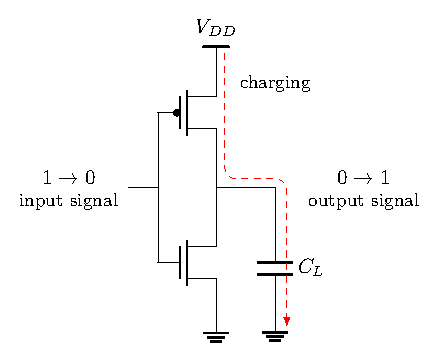
\includegraphics[width=0.5\textwidth]{fig/_TikZ__CMOS_charging.pdf} & 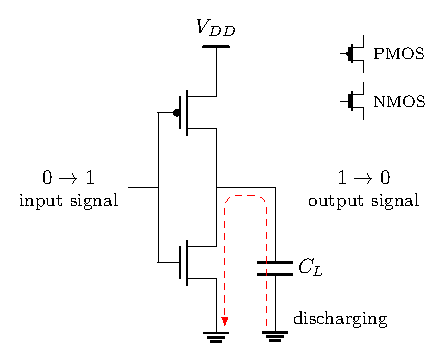
\includegraphics[width=0.5\textwidth]{fig/_TikZ__CMOS_discharging.pdf} \\
        (a) & (b)
    \end{tabular}
    \caption{Switching of the CMOS circuit, showing: (a) the charging path from $V_{DD}$ to $C_L$; (b) the discharging path $C_L$ to $GND$ of the capacitive load.}
    \label{fig:cmos}
\end{figure}
\end{frame}